\documentclass[11pt]{article}
\usepackage[letterpaper,margin=1in]{geometry}
\usepackage[T1]{fontenc}
\usepackage{lmodern,microtype,amsmath,amssymb,amsthm,booktabs,tabularx,graphicx}
\usepackage[hidelinks]{hyperref}
\hypersetup{%
  pdftitle={From enzyme activity to functional recovery: kinetic guarantees, sharp population bounds and measurement requirements},
  pdfsubject={Identified sets for a finite-time recovery task under pooled and calibrated enzyme observations},
  pdfkeywords={partial identification, enzyme kinetics, population heterogeneity, first passage time, sharp bounds, measurement design, formal verification}}

\newtheorem{theorem}{Theorem}[section]
\newtheorem{proposition}[theorem]{Proposition}
\newtheorem{corollary}[theorem]{Corollary}
\newtheorem{lemma}[theorem]{Lemma}
\theoremstyle{definition}
\newtheorem{example}[theorem]{Example}
\newtheorem{remark}[theorem]{Remark}

\newcommand{\E}{\mathbb E}
\newcommand{\R}{\mathbb R}
\newcommand{\ind}{\mathbf 1}
\newcommand{\code}[1]{\texttt{\small #1}}
\setlength{\emergencystretch}{2em}
\renewcommand{\topfraction}{0.92}
\renewcommand{\bottomfraction}{0.7}
\renewcommand{\textfraction}{0.07}
\renewcommand{\floatpagefraction}{0.85}
\newcommand{\horizonrows}{%
60 & 1.26730622 & 0.00000000 & 0.58383367 \\
120 & 0.95060185 & 0.11639578 & 1.00000000 \\
240 & 0.79237408 & 0.35636231 & 1.00000000 \\
1000 & 0.67309407 & 0.46574037 & 1.00000000 \\
}


\title{From enzyme activity to functional recovery:\\
kinetic guarantees, sharp population bounds\\ and measurement requirements}
\author{}
\date{16 September 2026}

\begin{document}
\maketitle

\begin{abstract}
An enzyme assay reports a rate. A recovery claim concerns a trajectory. A
population guarantee concerns how many trajectories complete a task. We treat
these as three distinct objects and compute what each observation certifies
about the next. For a prescribed, G6PD-inspired kinetic family we show that a
finite nonnegative dual certificate on observed rate bands implies literal
solutions and a \emph{uniform} arrival deadline for every
observation-compatible parameter vector, and we exhibit a parameter sequence
along which every member eventually recovers while no common deadline exists.
For finite weighted populations that differ only in catalytic capacity, with
mean capacity one and support $[5/8,9/14]\cup[1,11/8]$, the set of fractions
reaching the target by time $120$ is exactly $[20/41,1]$, although every such
population has the \emph{same entire} pooled clamped initial-rate response
surface; a calibrated classification readout narrows the exact set to
$[33/49,4/5]$, and one three-capacity construction realizes every value in
both sets. These claims, including solution existence, are verified in Lean 4,
as are the resulting minimax constants, the decision rule, and the
weighting conversion. Ordinary analysis then quantifies what the modelling
assumptions contribute: removing the support gap replaces the lower endpoint
by an unattained infimum near $.1164$; allowing a fraction $\eta$ of off-band
capacity gives a sharp interpolating infimum; equal mean and equal variance
still permit recovery fractions $1/4$ and $3/4$; readout error and cell-weight
normalization draw on one exactly computable margin; and the deadline-free
limit of the guarantee is $197/407<1/2$, approached at the exponential rate
$9/8470$ per unit model time with an explicitly identified prefactor. A
row-span criterion decides when a further assay can help at all, and a
monotone comparison theorem, together with a positive two-state
counterexample, delimits transfer of the scalar threshold to multidimensional
models. All numerical inputs are designed model values. The results specify
measurement requirements; they do not supply a clinically calibrated recovery
predictor.
\end{abstract}

\noindent\textbf{Keywords.} partial identification; enzyme kinetics;
population heterogeneity; first passage time; sharp bounds; measurement
design; formal verification.

\section{Introduction}\label{sec:intro}
An average activity assay summarizes rates. A recovery question counts cells
that complete a task under a stated load and deadline. A population can hold
enough high-capacity cells to maintain its mean while many other cells miss
that deadline, so the inferentially relevant object is not a point estimate but
the full set of recovery fractions compatible with the observations and the
kinetic assumptions. Writing $\mathcal C(y)$ for the class of models,
populations and nuisance parameters compatible with an observation $y$, and
$J(M)$ for the functional outcome of a member $M$, that object is the
identified set
\begin{equation}\label{eq:identified}
  \mathcal I(y)=\{J(M):M\in\mathcal C(y)\}.
\end{equation}
A guarantee must hold on all of $\mathcal I(y)$; a bound is sharp when it is
attained, or approached, by compatible witnesses; and a further measurement is
useful exactly when it cuts the class in a direction that moves the endpoints.
This is standard partial-identification reasoning
\cite{manski,tamer,bertsimas}, and we claim no novelty for the framework. What
we supply is a complete worked chain for one declared kinetic law: from rate
observations to actual solutions, from actual solutions to a population
identified set with explicit extremal witnesses, and from there to a
measurement specification, with the central implications machine-checked.

Glucose-6-phosphate dehydrogenase (G6PD) supplies the motivating vocabulary.
G6PD deficiency is common and clinically consequential \cite{luzzatto}, its
activity is measured both in bulk and cell by cell \cite{shah,kalnoky}, and
the expression mosaic in heterozygotes makes population heterogeneity concrete
rather than hypothetical. A kinetic study of redox imbalance after oxidative
crisis in G6PD-deficient erythrocytes \cite{shimo} supplies the functional
form of the rate law we use. None of these studies calibrates the particular
task defined below, and we do not claim that they do. The general warning that
population averages can conceal heterogeneity is also long established in cell
biology \cite{altschuler}; our contribution is quantitative, not
admonitory.

\subsection*{What this paper establishes}
Section~\ref{sec:model} fixes the rate law, the scalar task, the population
class, the pooled observation model and the unit conventions, and separates
three meanings of ``reserve'' that must not be conflated.

Section~\ref{sec:individual} treats a single cell whose six kinetic
coefficients are constrained by rate bands. In reciprocal coordinates the
class is a polyhedron, and a finite nonnegative dual certificate on the target
state yields a lower bound on the target rate. Theorem~\ref{thm:individual}
turns such a certificate into literal solutions of the original rate law and a
uniform arrival deadline valid for every compatible coefficient vector.
Example~\ref{ex:design} works out an observation design in exact rational
arithmetic; Remark~\ref{rem:nonuniform} shows that pointwise eventual recovery
of every class member does not give a common deadline, so a positive uniform
margin is not a technical convenience but the content of the statement.

Section~\ref{sec:main} contains the principal population result.
Theorem~\ref{thm:main} determines two exact identified sets for the recovery
fraction under a mean activity constraint and a designed separated support:
$[20/41,1]$ from bulk information, and $[33/49,4/5]$ after a calibrated binary
readout, with one three-capacity family realizing every value in each. The
pooled obstruction is stronger than a coincidence of one assay number: all
admitted populations share their entire clamped initial-rate response surface.

Section~\ref{sec:decision} converts the sets into decision statements: the
unavoidable minimax error, the readout precision needed for a designed
two-thirds performance requirement, the conversion between weighted and
number fractions, and---Proposition~\ref{prop:frontier}---an exact frontier
showing that readout error and weight normalization consume one shared margin.

Section~\ref{sec:support} isolates what the modelling assumptions contribute.
Proposition~\ref{prop:connected} removes the support gap and shows the lower
endpoint becomes an unattained infimum, bracketed by exact rational rectangle
sums; Proposition~\ref{prop:horizon} gives the deadline dependence and the
deadline-free limit $197/407$; Proposition~\ref{prop:asymptotic} identifies
the exponential rate and the exact constant governing approach to that limit;
and Proposition~\ref{prop:offband} interpolates between the designed gap and
connected support through a sharp off-band sensitivity parameter.

Section~\ref{sec:diagnostic} answers ``would another assay help?'' with a
row-span criterion (Proposition~\ref{prop:rowspan}) and an explicit case where
a second, nonlinear, correctly measured assay changes nothing.
Section~\ref{sec:multi} states conditions under which a scalar capacity
threshold survives in a multidimensional model, and a positive two-state
counterexample showing that cooperativity in the state alone does not suffice.
Section~\ref{sec:use} states the resulting measurement requirement, and
Section~\ref{sec:evidence} reports evidence scopes, formal declarations and
reproduction.

\subsection*{What this paper does not establish}
The principal theorem is deliberately small: one varying parameter, fixed
remaining kinetic inputs, finite nonnegative weights, no distributional fit, no
independence assumption and no numerical ODE solver in its proof. The support,
the load, the deadline and the readout calibration are designed mathematical
inputs, not estimates from a measured preparation. The scalar state is not a
full NADPH balance, and nothing here establishes simultaneous energy service,
peroxide control and whole-cell restart; erythrocyte models of that scope exist
and have different provenance \cite{nishino,rbcgem}. Machine verification
certifies the stated implications, not the biological adequacy of their
hypotheses.

\section{Model, task and observation semantics}\label{sec:model}

\subsection{Rate law and scalar specialization}
Consider the source rate
\begin{equation}\label{eq:source}
  v=\frac{V(N/K_n)(S/K_g)}
  {1+(N/K_n)(1+S/K_g)+H/K_h+A/K_a+B/K_b},
\end{equation}
whose functional form we take from the kinetic study \cite{shimo}: $V$ is a
catalytic capacity, $N$ and $S$ are substrate variables, and $H,A,B$ are
inhibitory species with affinities $K_h,K_a,K_b$. All kinetic parameters are
positive. For the population results we prescribe
\begin{equation}\label{eq:special}
  K_n=3,\quad K_g=S=7,\quad K_h=56,\quad K_a=125,\quad K_b=520,
  \qquad N=56-g,\ H=g,\ A=B=0,
\end{equation}
so that a single reduced-carrier coordinate $g$ both supplies the substrate
$N$ and inhibits through $H$. With a constant demand $q$ the task is
\begin{equation}\label{eq:ode}
  g'=V k(g)-q,\qquad
  k(g)=\frac{56-g}{115-(109/56)g},\qquad q=\frac3{10},\qquad g(0)=10 .
\end{equation}
The pool is $0\le g\le56$, the target is $g=28$, and the deadline is $T=120$.
Success means $g(t)\ge28$ for some $t$ in the \emph{closed} interval
$[0,120]$: arrival exactly at the deadline counts.

\subsection{Population class and the success functional}
A population consists of finitely many capacities $V_i$ with weights $w_i$,
\begin{equation}\label{eq:class}
  w_i\ge0,\quad \sum_iw_i=1,\quad \sum_iw_iV_i=1,\qquad
  V_i\in\mathcal S:=[5/8,9/14]\cup[1,11/8],
\end{equation}
and for any family of actual solutions of \eqref{eq:ode} on $[0,120]$ we write
\begin{equation}\label{eq:success}
  p=\sum_i w_i\ind\{\exists t\in[0,120]:g_i(t)\ge28\}.
\end{equation}
Real weights permit arbitrary convex mixtures; rational weights become cell
counts after clearing denominators, and in the worked interpretation of
Section~\ref{sec:use} the weights are cell numbers. Mean capacity one is a
reference normalization chosen for convenience, not a clinical category of
normal activity. Table~\ref{tab:notation} collects the notation used throughout.
Only $V$ varies across the population: the cells are
uncoupled and obey a common protocol, so no independence assumption is
involved anywhere except in the explicitly labelled sampling illustration of
Section~\ref{sec:decision}.

\subsection{Pooled clamped observations}
Under common clamped assay inputs $z=(N,S,H,A,B)$ the fixed affinities in
\eqref{eq:source} make the initial rate proportional to capacity,
$a(V;z)=V\psi(z)$ with $\psi(z)=a(1;z)$, so the pooled observation is
\begin{equation}\label{eq:pool}
  \bar a(z)=\sum_iw_ia(V_i;z)=\Big(\sum_iw_iV_i\Big)\psi(z)=\psi(z).
\end{equation}
This is an identity between functions of $z$, not the coincidence of one
number. Its interpretation is restricted to nonnegative input concentrations
and positive fixed kinetic parameters, and it presumes common clamping,
additive initial rates and consistent normalization. An intact-cell time
course with heterogeneous internal substrates is a different observation
model, and \eqref{eq:pool} says nothing about it.

\subsection{Units}
The constants in \eqref{eq:special}--\eqref{eq:ode} are model units. For a
pool $P$ and a reference rate $V_{\rm ref}$ on the same amount basis, writing
$x=g/P$, $\theta=V_{\rm ref}t/P$, $\nu=V/V_{\rm ref}$ and $\ell=q/V_{\rm ref}$
gives the dimensionless form $dx/d\theta=\nu k(Px)-\ell$, with $x_0=5/28$,
$x_R=1/2$ and $\theta_T=15/7$ at reference rate one. Restoring physical units
requires a matched pool, rate normalization, kinetic shape, load and time
scale. In particular $120$ is not asserted to mean $120$ minutes.

\begin{remark}[Three meanings of reserve]\label{rem:reserve}
A \emph{stock} reserve is a present amount of reduced carrier; a \emph{rate}
reserve is the ability to regenerate it relative to demand; a
\emph{functional} reserve is the ability to complete a stated task within a
stated horizon. Large stock can carry a transient despite slow regeneration,
and fast regeneration is useless without an available pool. In this paper $g$
is a stock coordinate, $V$ is a rate parameter, and \eqref{eq:success} is the
functional quantity. Carrier arrival at the target is not survival, viability,
membrane service or low oxidative burden, none of which is modelled here.
\end{remark}

\begin{remark}[Two levels of uncertainty]\label{rem:pooling}
Section~\ref{sec:individual} constrains the coefficients of \emph{one} cell;
Section~\ref{sec:main} constrains a \emph{mixture} of cells at the level of
rates. These do not compose naively. Reciprocal linearization is an
individual-realization statement, and for a heterogeneous mixture
$\bar v=\E[1/(\phi\cdot\beta)]$, whereas the reciprocal of the pooled rate is
$1/\bar v$, which differs from $\phi\cdot\E[\beta]$ in general. Applying an
individual reciprocal certificate to a pooled assay as though the pool were a
single kinetic realization is therefore invalid; a bridge between the two
levels is a substantive additional hypothesis, and we do not assert one.
\end{remark}

\begin{table}[ht]
\centering\small
\begin{tabularx}{\linewidth}{@{}ll>{\raggedright\arraybackslash}X@{}}
\toprule
Symbol & Meaning & Role and normalization\\
\midrule
$V$ & catalytic capacity & the only quantity varying across the population;
mean one by \eqref{eq:class}\\
$g$ & reduced-carrier coordinate & scalar state in $[0,56]$; stock, not a
whole-cell state\\
$q$ & demand & constant load $3/10$ in model units\\
$T$ & deadline & $120$ in model units unless stated; closed interval\\
$p$ & recovery fraction & weighted mass of cells with an actual hit of $28$ by
$T$\\
$s,f$ & readout sensitivity, false-positive rate & positive-readout fractions
\emph{within} the successful and failing classes for the task
\eqref{eq:success}\\
$r$ & observed positive fraction & $r=sp+f(1-p)$, no independence assumed\\
$R_h$ & cell-weight ratio & largest over smallest positive cell weight, used
to convert weighted to number fractions\\
$\beta,\phi$ & reciprocal coefficients, features & $1/v=\phi\cdot\beta$ for one
cell, Section~\ref{sec:individual}\\
$c_T$ & capacity cutoff at deadline $T$ & connected support only; $V_\infty$
is the deadline-free threshold\\
$\eta$ & off-band mass & weight violating the designed support gap,
Proposition~\ref{prop:offband}\\
\bottomrule
\end{tabularx}
\caption{Notation. Sensitivity and specificity here refer to the functional
task \eqref{eq:success}, not to any clinical G6PD deficiency
label.}\label{tab:notation}
\end{table}

\section{From kinetic observations to individual recovery}\label{sec:individual}

\subsection{Reciprocal coordinates}
Fix $N,S>0$ and put
\begin{equation}\label{eq:coords}
  \beta=\Big(\frac1V,\frac{K_g}V,\frac{K_nK_g}V,
  \frac{K_nK_g}{VK_h},\frac{K_nK_g}{VK_a},\frac{K_nK_g}{VK_b}\Big),
  \qquad
  \phi=\Big(1,\frac1S,\frac1{NS},\frac H{NS},\frac A{NS},\frac B{NS}\Big).
\end{equation}
Expanding \eqref{eq:source} gives $1/v=\phi\cdot\beta$. The map
\eqref{eq:coords} from positive parameters to positive coefficients is a
bijection, with inverse
\begin{equation}\label{eq:inverse}
  (V,K_g,K_n,K_h,K_a,K_b)
  =\Big(\frac1{\beta_0},\frac{\beta_1}{\beta_0},\frac{\beta_2}{\beta_1},
  \frac{\beta_2}{\beta_3},\frac{\beta_2}{\beta_4},\frac{\beta_2}{\beta_5}\Big).
\end{equation}
Consequently a band $v\in[v_-,v_+]$ with $v_->0$ observed at inputs
$(N,S,H,A,B)$ is exactly the pair of linear inequalities
$1/v_+\le\phi\cdot\beta\le1/v_-$, and an observation class described by finitely
many such bands is a polyhedron in $\beta$. Working in $\beta$ therefore
replaces a nonlinear parameter-estimation problem by linear programming
duality, without leaving the original kinetic family: every positive $\beta$ is
the coefficient vector of an actual parameter vector through
\eqref{eq:inverse}.

With $N=P-g$, $H=g$ and $S,A,B$ fixed, \eqref{eq:coords} collapses to
\begin{equation}\label{eq:scalarrate}
  v(g)=\frac{P-g}{a(P-g)+bg+c},\qquad
  a=\beta_0+\frac{\beta_1}S,\quad b=\frac{\beta_3}S,\quad
  c=\frac{\beta_2+\beta_4A+\beta_5B}S,
\end{equation}
with $a,b,c>0$, and the target-state reciprocal rate is
$1/v(R)=\phi_R\cdot\beta$ for the feature vector $\phi_R$ of
\eqref{eq:coords} evaluated at $N=P-R$, $H=R$.

\begin{lemma}[Exact secant identity]\label{lem:secant}
For $a,b,c>0$ and $0\le x<y\le P$, with $D(g)=a(P-g)+bg+c>0$,
\begin{equation}\label{eq:secant}
  v(x)-v(y)=\frac{(bP+c)(y-x)}{D(x)D(y)}>0 .
\end{equation}
\end{lemma}
\begin{proof}
$D>0$ on $[0,P]$ because it is affine with positive values
$aP+c$ and $bP+c$ at the endpoints. Clearing denominators,
$(P-x)D(y)-(P-y)D(x)=b\,[y(P-x)-x(P-y)]+c(y-x)=(bP+c)(y-x)$.
\end{proof}

So $v$ is strictly decreasing: the state both feeds and inhibits, and
inhibition wins uniformly. Two consequences are used repeatedly. First, the
drift $v-q$ is smallest at the target among all states below it, so a bound at
the target bounds the whole approach. Second, arrival is decided by the sign of
the target drift, with no need for a long numerical run.

\subsection{A certificate that implies a uniform deadline}

\begin{theorem}[Certified individual recovery]\label{thm:individual}
Let $P>0$, $S>0$, $A,B\ge0$, $q>0$ and $0\le x<R<P$. Let $F_i\in\R^6$ and
$b_i\in\R$, $i$ in a finite index set, describe an observation class
$\{\beta>0:F_i\cdot\beta\le b_i\ \forall i\}$. Suppose there are multipliers
$y_i\ge0$ and a number $U>0$ with
\begin{equation}\label{eq:cert}
  \sum_iy_iF_i=\phi_R,\qquad \sum_iy_ib_i\le U,\qquad q<\frac1U .
\end{equation}
Then for \emph{every} positive $\beta$ in the class the initial value problem
$g'=v(g)-q$, $g(0)=x$, with $v$ the literal rate \eqref{eq:source} at the
parameters \eqref{eq:inverse} and inputs $N=P-g$, $H=g$, has a solution that
remains in $[0,P]$ and satisfies
\begin{equation}\label{eq:deadline}
  g(t^\star)\ge R\quad\text{for some } t^\star\le\frac{R-x}{1/U-q}.
\end{equation}
\end{theorem}
\begin{proof}
Fix a compatible $\beta$ and let $a,b,c$ be as in \eqref{eq:scalarrate}; they
are positive. Nonnegative combination of the observed inequalities gives
$\phi_R\cdot\beta=\sum_iy_iF_i\cdot\beta\le\sum_iy_ib_i\le U$, that is
$v(R)\ge1/U$, hence the target drift is at least $m:=1/U-q>0$. By
Lemma~\ref{lem:secant}, $v(g)\ge v(R)$ for all $g\le R$, so
\begin{equation}\label{eq:driftbound}
  v(g)-q\ge m>0\qquad (0\le g\le R).
\end{equation}
In particular $v(0)\ge q$, so the field points inward at $g=0$; at $g=P$ it
equals $-q<0$. The field is locally Lipschitz on $[0,P]$ because $D$ is
bounded away from zero there. Local existence, uniqueness and continuation,
together with forward invariance of $[0,P]$, give a solution on every finite
horizon; equivalently, extend the field to a globally bounded Lipschitz field
agreeing with it on $[0,P]$, solve, and observe that the solution never leaves
$[0,P]$, so it solves the original problem. Suppose $g(t)<R$ for all
$t\in[0,\bar t\,]$ with $\bar t=(R-x)/m$. Then \eqref{eq:driftbound} applies
throughout, and integrating gives $g(\bar t\,)\ge x+m\bar t=R$, a
contradiction. Hence \eqref{eq:deadline} holds. Finally, the rate used in the
argument is the literal \eqref{eq:source} at the parameters \eqref{eq:inverse},
including at the pool boundary, by the reciprocal expansion of
Section~\ref{sec:individual}.
\end{proof}

Theorem~\ref{thm:individual} is the composition that matters for experiment
design: the observations are constraints, the multipliers are a proof, and the
output is a deadline. A numerical optimizer may propose $y$; exact arithmetic
then checks \eqref{eq:cert}, and no property of the optimizer is used
afterwards. A feasible positive $\beta$ certifies in addition that the class is
nonempty, which is what makes the conclusion non-vacuous.

\begin{example}[An observation design]\label{ex:design}
Take $P=56$, $q=3/10$, $x=10$, $R=28$, and a class in which $a=2$, $c=3$ are
pinned and only the inhibition coefficient varies, $b=3/K$ with $K>0$ unknown.
Then $1/v(28)=(59+84/K)/28$, so the exact decision boundary is
\[
  v(28)>q\iff K>\frac{252}{103}.
\]
Suppose the available inhibitory observation is the designed functional
$y(K)=K/(3K+56)$, increasing in $K$, so that the decision boundary reads
$y>9/233$. An observed band $y\in[.24,.26]$ is the interval
$K\in[48,728/11]$ and yields the exact conclusions in
Table~\ref{tab:design}: a worst-case target reciprocal rate $243/112$,
a guaranteed target drift $391/2430$, and the uniform deadline
$43740/391\approx111.8670$ for every compatible $K$ in the band.
\end{example}

\begin{table}[ht]
\centering
\begin{tabular}{@{}lr@{}}
\toprule
Quantity & Value\\
\midrule
Decision boundary in the unknown coefficient & $K>252/103$\\
Equivalent boundary in the observed functional & $y>9/233$\\
Designed observation band & $y\in[.24,.26]$\\
Worst-case target reciprocal rate on the band & $243/112$\\
Guaranteed target rate & $112/243$\\
Guaranteed target drift & $391/2430$\\
Uniform arrival deadline & $43740/391\approx111.8670$\\
A compatible realization & $K=56$, $y=1/4$\\
First passage time of that realization & $\approx103.8058$ (numerical)\\
\bottomrule
\end{tabular}
\caption{Exact consequences of the designed band in Example~\ref{ex:design}.
The band is an illustrative design, not a same-preparation measurement. Only
the last row is numerical.}\label{tab:design}
\end{table}

Two features of Example~\ref{ex:design} deserve emphasis. First, without an
observation that constrains the inhibition direction, the class contains
$\beta$ with arbitrarily large $b$, and the worst-case target rate tends to
zero: no amount of extra precision in the \emph{remaining} coordinates repairs
this, because those coordinates do not appear in the missing direction. This is
structural rather than statistical non-identifiability, and it is visible
before any data are seen; profile-likelihood diagnostics address the practical
variant of the same question for fitted models \cite{raue}. The useful
experimental question is which observation sees the direction that the task
depends on. Second, the compatible realization $K=56$ is not an
incidental choice: it gives $b=3/56$, hence
$v(g)=(56-g)/(2(56-g)+(3/56)g+3)=k(g)$, which is exactly the capacity-one cell
of \eqref{eq:ode}. The individual and population parts of this paper therefore
concern the same scalar law, approached from two different observation models.

\begin{remark}[Eventual recovery without a uniform deadline]\label{rem:nonuniform}
Let $K\downarrow252/103$ within the class of Example~\ref{ex:design}. Every
member has positive target drift, hence recovers in finite time by
Theorem~\ref{thm:individual} applied to its own singleton class, but the drift
margin tends to zero and the arrival times diverge. Pointwise eventual
recovery of every member of a noncompact class therefore does not produce one
finite deadline for the class. A uniform statement needs a positive uniform
margin, as in \eqref{eq:cert}, or a separate uniform passage-time argument.
\end{remark}

\section{The sharp population theorem}\label{sec:main}

\begin{theorem}[Exact bulk and repaired identified sets]\label{thm:main}
Every population satisfying \eqref{eq:class} admits solutions of
\eqref{eq:ode} on $[0,120]$ that remain in $[0,56]$. For every such family of
actual solutions:
\begin{enumerate}
\item its recovery fraction \eqref{eq:success} satisfies $20/41\le p\le1$;
\item its entire pooled clamped response surface is $\bar a(z)=\psi(z)$;
\item if $r=sp+f(1-p)$ and
\begin{equation}\label{eq:readout}
  \frac9{10}\le s\le1,\qquad 0\le f\le\frac1{50},\qquad
  \frac{17}{25}\le r\le\frac{18}{25},
\end{equation}
then $33/49\le p\le4/5$.
\end{enumerate}
Conversely, every value in $[20/41,1]$ is realized by an admitted population
together with actual solutions, and every value in $[33/49,4/5]$ is realized in
the same class with readout parameters satisfying \eqref{eq:readout}. At most
three positive-weight capacities are needed for either family.
\end{theorem}

The readout quantities are conditional rates for the actual task
\eqref{eq:success}: $s$ is the positive-readout fraction among successful
cells, $f$ the positive-readout fraction among failing cells, and $r$ the
overall positive fraction. The mixture identity $r=sp+f(1-p)$ is a
decomposition of a total mass, not an independence assumption; if a class has
zero mass one works with joint masses and no conditional ratio. The calibration
bounds \eqref{eq:readout} are designed inputs.

\subsection{Existence and classification}
The denominator of $k$ is affine and positive on $[0,56]$, with value $115$ at
$g=0$ and $6$ at $g=56$. For every admitted capacity,
\[
  Vk(0)-q\ge\frac58\cdot\frac{56}{115}-\frac3{10}=\frac1{230}>0,
  \qquad Vk(56)-q=-\frac3{10}<0,
\]
so the field points inward at both ends of the pool, and the argument of
Theorem~\ref{thm:individual} gives solutions on $[0,120]$ staying in $[0,56]$,
unique by local Lipschitz continuity. Moreover
\begin{equation}\label{eq:derivative}
  k'(g)=-\frac6{(115-(109/56)g)^2}<0,\qquad Vk(28)=\frac{56V}{121},
\end{equation}
which is Lemma~\ref{lem:secant} in the present normalization.

A low-band cell, $V\le9/14$, has target drift at most
$\tfrac9{14}\cdot\tfrac{56}{121}-\tfrac3{10}=-\tfrac3{1210}<0$. It cannot
cross the target: at a first hit from below a differentiable trajectory would
have nonnegative left derivative, contradicting the strictly negative
prescribed derivative there. A high-band cell, $V\ge1$, has drift at least
$\tfrac{56}{121}-\tfrac3{10}=\tfrac{197}{1210}$ while below the target by
\eqref{eq:derivative}, so if no hit had occurred by
\begin{equation}\label{eq:T0}
  T_0=\frac{28-10}{197/1210}=\frac{21780}{197}\approx110.5584<120,
\end{equation}
integrating the drift bound would force $g(T_0)\ge28$, a contradiction. Hence
for every admitted capacity and every admitted trajectory
\begin{equation}\label{eq:classify}
  \exists t\in[0,120]:g(t)\ge28\quad\Longleftrightarrow\quad V\ge1 .
\end{equation}
Success is therefore membership in the upper band, for all solutions
simultaneously; the designed support gap is what makes the classification this
clean, and Section~\ref{sec:support} quantifies its role.

\subsection{Averaging, compensation and sharpness}
Let $I=\ind\{V\ge1\}$. On the support $\mathcal S$ the pointwise bound
\begin{equation}\label{eq:majorant}
  V\le\frac9{14}+\frac{41}{56}I
\end{equation}
holds, with equality exactly at the two capacities $9/14$ and $11/8$. Taking
expectations and using $\E[V]=1$ gives $1\le\frac9{14}+\frac{41}{56}p$, that
is $p\ge20/41$; normalization gives $p\le1$; and \eqref{eq:pool} gives the
response-surface identity. The mechanism is a compensation budget: a population
can hide failing cells only if its successful cells make up the capacity
deficit, and the largest admitted successful capacity caps how much
compensation a unit of successful mass can supply.

That reading dictates the extremal construction. To make $p$ as small as
possible, failing mass should be as heavy as failing mass may be, hence at the
largest failing capacity $9/14$; and the compensating successful mass should be
as efficient as possible, hence at the largest successful capacity $11/8$. Two
atoms already give the endpoint, with weights $21/41$ at $9/14$ and $20/41$ at
$11/8$. A third atom exactly at the mean, $V=1$, is neutral for the mean
constraint and successful for the task, so any amount of it can be substituted
in to raise $p$ continuously to one. Concretely, for $p\in[20/41,1]$ put
\begin{equation}\label{eq:witness}
  \Big(1-p,\ \frac{20(1-p)}{21},\ \frac{41p-20}{21}\Big)
  \quad\text{at capacities}\quad\Big(\frac9{14},\frac{11}8,1\Big).
\end{equation}
The weights are nonnegative on the whole interval, they sum to one, the mean
capacity is one, and the high-band mass is $p$. By \eqref{eq:classify} and the
existence statement these are dynamical witnesses, not distributions to which
success labels have been assigned by fiat. A count realization at the lower
endpoint is $42$ cells at $9/14$ and $40$ at $11/8$.

\subsection{Measurement repair and joint feasibility}
For $0\le p\le1$ the calibration bounds \eqref{eq:readout} give
$\tfrac9{10}p\le r\le\tfrac1{50}+\tfrac{49}{50}p$, which with
$17/25\le r\le18/25$ yields
\begin{equation}\label{eq:repaired}
  \frac{33}{49}\le p\le\frac45 .
\end{equation}
Necessary inequalities alone would not prove sharpness: kinetics, the mean
constraint and the readout must be satisfiable \emph{simultaneously}. Take the
witness \eqref{eq:witness} and set
\begin{equation}\label{eq:calibration-witness}
  (s,f,r)=
  \begin{cases}
  \big(1,\ (17/25-p)/(1-p),\ 17/25\big), & 33/49\le p\le17/25,\\[2pt]
  \big(1,\ 0,\ p\big), & 17/25\le p\le18/25,\\[2pt]
  \big((18/25)/p,\ 0,\ 18/25\big), & 18/25\le p\le4/5 .
  \end{cases}
\end{equation}
In the first branch the readout is perfectly sensitive and the observed total
is held at its lower bound by admitting exactly enough false positives; the
required $f$ is nonnegative and at most $1/50$ precisely on that
subinterval. In the middle branch the readout is perfect in both directions, so
$r=p$, which lies in the observed band there. In the third branch there are no
false positives and sensitivity is reduced to hold $r$ at its upper bound;
$(18/25)/p\ge9/10$ exactly when $p\le4/5$. Each branch therefore satisfies
every bound in \eqref{eq:readout} on its portion of \eqref{eq:repaired}, so the
same mean-constrained kinetic population supplies the readout. For an explicit
binary-labelled population, split each capacity atom into positive- and
negative-readout atoms in the conditional proportions just computed; this
leaves capacities and trajectories unchanged and uses at most three distinct
capacities with at most six labelled atoms. This proves
Theorem~\ref{thm:main}.

\begin{figure}[ht]
\centering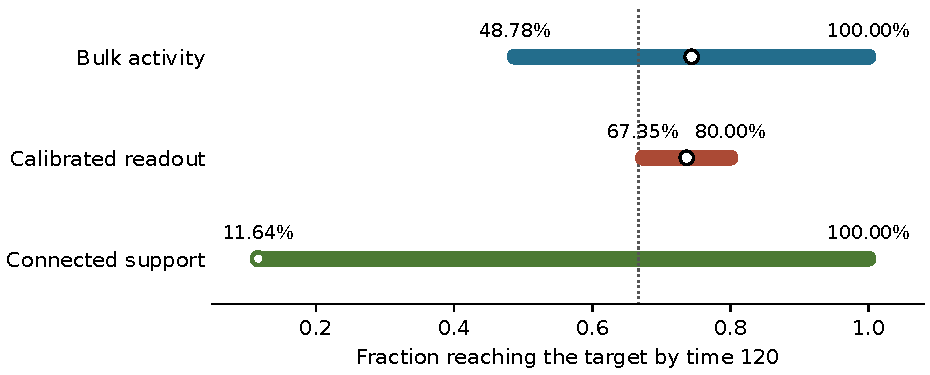
\includegraphics[width=\linewidth]{figures/identified_intervals.pdf}
\caption{Exact sets of compatible recovery fractions. Filled endpoints are
attained and white points mark minimax midpoints; the open endpoint of the
connected-support set (Proposition~\ref{prop:connected}) is an unattained
infimum. The dotted line is the designed two-thirds requirement. These are
identified sets for the stated assumptions, not statistical confidence
intervals.}\label{fig:intervals}
\end{figure}

\section{Decision consequences}\label{sec:decision}

\subsection{Unavoidable estimation error}
\begin{corollary}[Absolute-error limits]\label{cor:minimax}
Any estimate of $p$ based only on the bulk information in
Theorem~\ref{thm:main} has worst-case absolute error at least $21/82$, and the
midpoint $61/82$ attains that bound. Under the interval-valued readout
information \eqref{eq:readout} the optimal midpoint and worst-case error are
$361/490$ and $31/490$.
\end{corollary}
\begin{proof}
For an identified interval $[L,U]$ and any estimate $\hat p$, the triangle
inequality gives $U-L\le|U-\hat p|+|\hat p-L|$, so one of the two endpoint
errors is at least $(U-L)/2$; both endpoints are attained by
Theorem~\ref{thm:main}. Conversely the midpoint has error at most $(U-L)/2$
everywhere on the interval. Substituting the two intervals gives the
constants.
\end{proof}

The two radii are about $25.61$ and $6.33$ percentage points of recovery, a
reduction of roughly $75.3\%$ in identified-set width. They are not sampling
standard errors, and they cannot be reduced by measuring the same pooled
quantity more precisely: a deterministic procedure must return the same value
for two populations whose observations are identical, and by
Theorem~\ref{thm:main} such pairs differ in recovery fraction by up to
$21/41$. Reporting an exact readout value rather than the interval
\eqref{eq:readout} would define a smaller class and a different, smaller radius.

\subsection{A precision requirement for a performance target}
If $s\le s_+$, $f\le f_+$ and $s_+>f_+$, then $r\le f_++(s_+-f_+)p$, so a
lower readout bound $r_-$ certifies $p\ge p_*$ whenever
\begin{equation}\label{eq:decision}
  r_-\ge f_++(s_+-f_+)p_* .
\end{equation}
For the designed requirement $p_*=2/3$ with $s_+=1$, $f_+=1/50$ the threshold
is $101/150$, and the available bound $17/25$ leaves
\begin{equation}\label{eq:budget}
  \frac{17}{25}-\frac{101}{150}=\frac1{150},\qquad
  \frac{33}{49}-\frac23=\frac1{147}.
\end{equation}
These two numbers are different quantities: the first is the additional
downward readout error the certificate tolerates, the second is the slack in
the certified recovery fraction itself. Replacing $r_-$ by $17/25-\varepsilon$
preserves the non-strict two-thirds guarantee exactly for
$\varepsilon\le1/150$. Uncertainty already included in \eqref{eq:readout} must
not be subtracted twice, and improving only the lower sensitivity bound moves
the \emph{upper} recovery bound, not this lower certificate. Two-thirds is a
designed performance requirement used to exhibit decision sensitivity; it is
not a clinical threshold.

As a transparent sampling illustration, suppose one positive-readout
proportion is estimated from $n$ independent representative Bernoulli draws.
Hoeffding's inequality \cite{hoeffding} gives one-sided error
$\varepsilon_n=\sqrt{\log(1/\delta)/(2n)}$ at confidence $1-\delta$; at
$\delta=.05$, requiring $\varepsilon_n\le1/150$ gives the conservative
sufficient count $n\ge33{,}702$, and controlling both sides of that one
proportion gives $41{,}500$. These are model precision calculations under an
assumed sampling model, not clinical sample-size recommendations: cell
clustering, donor-level sampling, gating selection and systematic calibration
error each require separate treatment.

\subsection{Normalization can consume the margin}
\begin{proposition}[Change of population weights]\label{prop:weights}
Suppose a justified observation model supplies a weighted successful fraction
$r_h$, and that positive cell weights have ratio at most $R_h\ge1$. Then the
number fraction $p_n$ satisfies
\begin{equation}\label{eq:weights}
  \frac{r_h}{R_h(1-r_h)+r_h}\le p_n\le\frac{R_hr_h}{1-r_h+R_hr_h},
\end{equation}
and the weighted interval $[33/49,4/5]$ gives the number-fraction enclosure
\begin{equation}\label{eq:weighted-repair}
  \Big[\frac{33}{33+16R_h},\ \frac{4R_h}{1+4R_h}\Big],
\end{equation}
whose lower endpoint is at least $2/3$ exactly when $R_h\le33/32$. At
$R_h=6/5$ the enclosure is $[55/87,24/29]\approx[63.22\%,82.76\%]$.
\end{proposition}
\begin{proof}
Divide all weights by their smallest positive value, so each lies in
$[1,R_h]$. On a number-normalized population let $A$ and $B$ be the successful
and failing weighted masses. Then $p_n\le A\le R_hp_n$ and
$1-p_n\le B\le R_h(1-p_n)$, and $r_h=A/(A+B)$. Extremizing the ratio gives
\[
  \frac{p_n}{p_n+R_h(1-p_n)}\le r_h\le\frac{R_hp_n}{R_hp_n+1-p_n},
\]
and inverting these Möbius maps, which are increasing in $p_n$, gives
\eqref{eq:weights}. Both bounds in \eqref{eq:weights} increase in $r_h$, since
their derivatives have numerator $R_h>0$; substituting the endpoints of
$[33/49,4/5]$ gives \eqref{eq:weighted-repair}, and clearing positive
denominators proves the remaining claims.
\end{proof}

At $R_h=6/5$ the converted lower endpoint no longer certifies two-thirds.
Proposition~\ref{prop:weights} converts a weighted \emph{success fraction};
it does not convert a mean activity in U/g Hb into a recovery fraction, for
which a separate justified map is needed. If capacities, weights and
calibration are coupled by further constraints, \eqref{eq:weights} remains
valid, but sharpness would have to be re-established with those constraints
imposed jointly. No conversion is needed when the observation and the target
are already number weighted.

\subsection{One margin, two claimants}
\begin{proposition}[Exact error--normalization frontier]\label{prop:frontier}
Keep $s_+=1$, $f_+=1/50$, replace the lower readout bound by
$17/25-\varepsilon$ with $\varepsilon\ge0$, and let
$\alpha(\varepsilon)=(33-50\varepsilon)/49$ be the resulting weighted lower
bound, assumed to lie in $[0,1]$. For a cell-weight ratio $R_h\ge1$, the
composed certificate $p_n\ge2/3$ obtained by applying
Proposition~\ref{prop:weights} to $\alpha(\varepsilon)$ holds if and only if
\begin{equation}\label{eq:frontier}
  \varepsilon\le\frac{33-32R_h}{50(1+2R_h)} .
\end{equation}
In particular the budget is $1/150$ at $R_h=1$, only $9/3800\approx.0023684$
at $R_h=51/50$, and empty for $R_h>33/32$.
\end{proposition}
\begin{proof}
By \eqref{eq:decision} with $r_-=17/25-\varepsilon$ the weighted bound is
$\alpha(\varepsilon)$. By \eqref{eq:weights} the converted lower endpoint is at
least $2/3$ iff $3\alpha\ge2R_h(1-\alpha)+2\alpha$, i.e.\ iff
$\alpha\ge2R_h/(1+2R_h)$. Substituting $\alpha=(33-50\varepsilon)/49$ and
clearing the positive denominators $49(1+2R_h)$ gives
$33-32R_h\ge50\varepsilon(1+2R_h)$, which is \eqref{eq:frontier}.
\end{proof}

Independent error allowances therefore cannot each consume the whole original
margin: they are claims on one exactly computable budget
(Figure~\ref{fig:frontier}). At $R_h=6/5$ the certificate would need a
weighted successful fraction of at least $12/17$, hence a lower positive-readout
bound of $121/170\approx.71176$, which the available $17/25=.68$ does not
supply. Proposition~\ref{prop:frontier} is an exact algebraic frontier for this
composed enclosure. It is not a claim that the two error sources are
biologically independent, and a joint model coupling weights to capacity would
need its own analysis.

\begin{figure}[ht]
\centering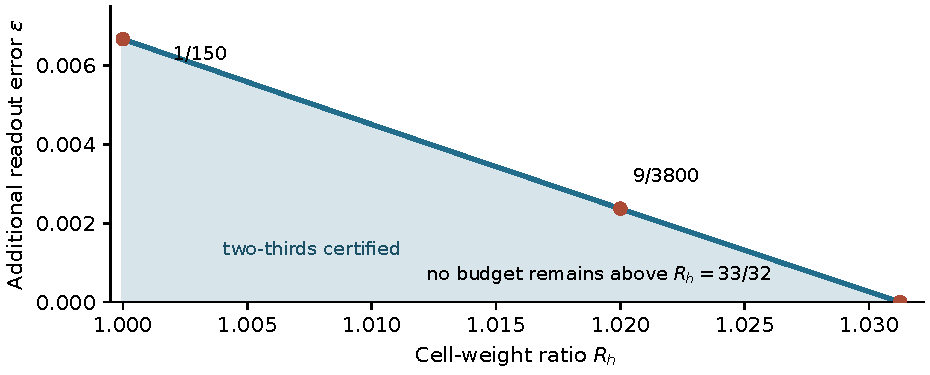
\includegraphics[width=\linewidth]{figures/margin_frontier.pdf}
\caption{The frontier \eqref{eq:frontier}. Inside the shaded region the
composed certificate still gives a number fraction of at least two-thirds.
The region closes at $R_h=33/32$, where weight normalization alone exhausts
the margin.}\label{fig:frontier}
\end{figure}

\section{What the support and deadline assumptions contribute}\label{sec:support}
The results of this section are ordinary mathematics, with the passage-time
brackets supported by exact rational arithmetic. They are not claimed as
machine-verified theorems; Table~\ref{tab:evidence} records the distinction.

\subsection{Longer horizons on the separated support}
For any $T\ge T_0$ from \eqref{eq:T0}, construct solutions of \eqref{eq:ode}
on the actual interval $[0,T]$ by the same compact-interval argument. Low-band
cells cannot hit on that interval, by the same first-hit contradiction.
Restricting a high-band solution to $[0,T_0]$ and applying the positive-drift
bound shows it hits by $T_0\le T$. Hence the successful fraction is again the
high-band mass, and the witnesses \eqref{eq:witness} prove the same exact
interval $[20/41,1]$ for every such horizon: on this support, waiting longer
removes none of the bulk ambiguity. This is a statement about solutions
constructed on $[0,T]$; it does not extrapolate a trajectory known only on
$[0,120]$.

\subsection{Connected support and the inclusive cutoff}
Now admit every capacity in $[a,d]=[5/8,11/8]$, keeping mean one, the same
load and the same task. The deadline-free threshold is
\begin{equation}\label{eq:Vinf}
  V_\infty=\frac q{k(28)}=\frac{363}{560}\approx.6482 .
\end{equation}
For $V>V_\infty$ the drift is positive up to the target, and the first passage
time is
\begin{equation}\label{eq:passage}
  \tau(V)=\int_{10}^{28}\frac{dg}{Vk(g)-q}.
\end{equation}
To justify \eqref{eq:passage} for an actual solution rather than as a
separation-of-variables ansatz, note that the primitive
$G(g)=\int_{10}^g(Vk-q)^{-1}$ satisfies $\frac{d}{dt}G(g(t))=1$ before the
first hit; the positive target drift supplies a hit by the argument of
Theorem~\ref{thm:individual}, and evaluating at the hitting time gives
\eqref{eq:passage}. For $V\le V_\infty$ no finite hit occurs: negative target
drift excludes first arrival, and in the equality case the target is an
equilibrium, which uniqueness forbids reaching from a different initial state.

The integrand is positive and strictly decreasing in $V$, and on a compact
neighbourhood of any $V>V_\infty$ its denominator is bounded away from zero, so
$\tau$ is continuous and strictly decreasing there. With
$B_0=109/56$, $\alpha=56V-115q$ and $\beta=V-qB_0>0$, partial fractions give
the closed form
\begin{equation}\label{eq:log}
  \tau(V)=\frac{18B_0}\beta+\frac{6V}{\beta^2}
  \log\frac{\alpha-10\beta}{\alpha-28\beta}.
\end{equation}
Since $\alpha-28\beta=28(V-V_\infty)$, the logarithm diverges as
$V\downarrow V_\infty$ while its numerator stays positive, so
$\tau(V)\to\infty$; and $\tau(V)\le18/(Vk(28)-q)\to0$ as $V\to\infty$. Hence
for each $T>0$ there is a unique cutoff $c_T>V_\infty$ with $\tau(c_T)=T$, and
success by $T$ is exactly $V\ge c_T$.

\begin{proposition}[Connected-support identified set at the deadline
$120$]\label{prop:connected}
Let $c=c_{120}$. Then $19/20<c<951/1000$, and the exact set of compatible
recovery fractions under mean one and support $[a,d]$ is
\begin{equation}\label{eq:connected}
  \Big(\frac{1-c}{11/8-c},\ 1\Big],
\end{equation}
whose lower endpoint is an infimum and is \emph{not} attained. The bracket
alone gives $49/424<\inf p<2/17$, and numerically
$c\approx.9506018463$, $\inf p\approx.1163957789$.
\end{proposition}
\begin{proof}
Since $k$ decreases, $h_V(g)=(Vk(g)-q)^{-1}$ increases on $[10,28]$ for
$V>V_\infty$, so for a uniform partition with $n=128$ the left and right
rectangle sums bracket \eqref{eq:passage} from below and above. For rational
$V$ these sums are rational and are evaluated exactly in
Table~\ref{tab:rectangles}; the rows $V=19/20$ and $V=951/1000$ give
$\tau(19/20)>120>\tau(951/1000)$, and monotonicity of $\tau$ gives the
bracket for $c$.

For validity, $I=\ind\{V\ge c\}$ satisfies $V\le c+(d-c)I$ on $[a,d]$, because
a failing capacity is below $c$ and a successful one is at most $d$; averaging
against mean one gives $p\ge(1-c)/(d-c)$, and normalization gives $p\le1$. For
sharpness, let $x\in[a,c)$ and mix atoms at $x$ and $d$ with successful weight
$p_x=(1-x)/(d-x)$, which has mean one; $p_x$ decreases to $(1-c)/(d-c)$ as
$x\uparrow c$. Mixing such a population with the uniform capacity-one
population attains every larger value up to one. Finally the endpoint is not
attained: equality in the averaged inequality requires every unit of failing
mass to sit exactly at $c$, where it would in fact succeed, and if there is no
failing mass equality requires all capacity at $d$, contradicting mean one.
\end{proof}

\begin{table}[ht]
\centering
\begin{tabular}{rrrl}
\toprule
Capacity $V$ & Lower passage bound & Upper passage bound & Hit by $120$?\\
\midrule
$19/20$ & 120.171857 & 120.285392 & No\\
$951/1000$ & 119.792912 & 119.905845 & Yes\\
$7/8$ & 157.558903 & 157.739481 & No\\
$9/8$ & 77.356392 & 77.411824 & Yes\\
$11/8$ & 51.267354 & 51.297023 & Yes\\
\bottomrule
\end{tabular}
\caption{Outward decimal roundings of exact rational left and right rectangle
sums with $128$ subintervals. Their reading as passage-time bounds uses the
ordinary argument for \eqref{eq:passage}; no numerical integration certificate
is involved, and the decimal value of $c_{120}$ is not a premise
anywhere.}\label{tab:rectangles}
\end{table}

\begin{figure}[ht]
\centering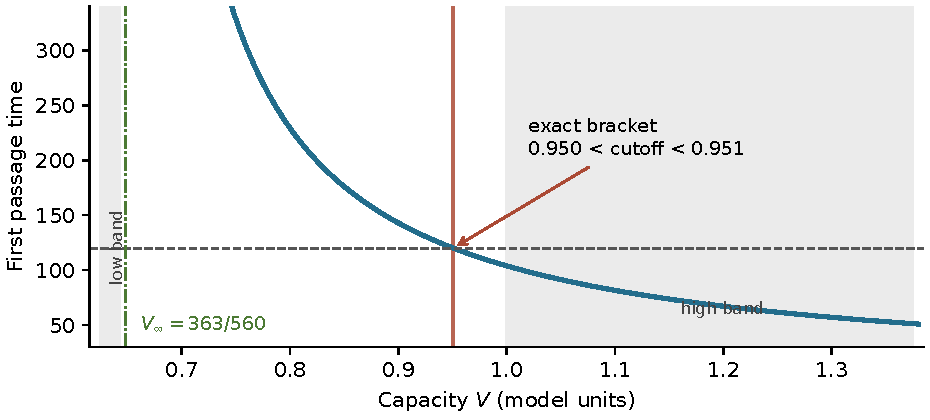
\includegraphics[width=\linewidth]{figures/passage_time.pdf}
\caption{First passage time \eqref{eq:passage} against capacity. Shaded
vertical strips are the two designed support bands of \eqref{eq:class}; the
gap between them is what makes the classification \eqref{eq:classify}
elementary. The plotted curve is a numerical evaluation; the marked cutoff has
the separate exact rational bracket $(.950,.951)$, and $V_\infty$ is the
deadline-free threshold \eqref{eq:Vinf}, at which $\tau$
diverges.}\label{fig:passage}
\end{figure}

The support gap does substantial inferential work: removing it moves the
guaranteed fraction from $20/41\approx.4878$ to an unattained infimum near
$.1164$, a far larger change than any improvement in the precision of an
already exact bulk mean. A small explicit example: $15$ cells at $V=19/20$ and
two at $V=11/8$ have mean one, but only the two recover by $120$, whereas all
$17$ cells of the uniform capacity-one population recover. The $15$ slower
cells do eventually recover; the deadline is essential to the example.

\subsection{Mean and variance do not identify the outcome}
The two connected-support populations
\begin{equation}\label{eq:variance}
  \mu_A=\tfrac34\delta_{7/8}+\tfrac14\delta_{11/8},\qquad
  \mu_B=\tfrac14\delta_{5/8}+\tfrac34\delta_{9/8}
\end{equation}
both have mean one and variance $3/64$, yet their recovery fractions are $1/4$
and $3/4$. Table~\ref{tab:rectangles} classifies the interior atoms $7/8$ and
$9/8$, and $5/8<V_\infty$ supplies the remaining failure. So adding a second
moment to the bulk information does not identify the recovery fraction on this
class; it does not follow that variance never tightens a bound, and
Section~\ref{sec:diagnostic} gives the criterion that decides such questions.

\subsection{Deadline dependence and the deadline-free limit}
\begin{proposition}[Sharp limits at a general deadline]\label{prop:horizon}
Fix mean one and support $[a,d]$. If $a<c_T<d$, the sharp lower and upper
limits of the recovery fraction are
\begin{equation}\label{eq:LU}
  L(T)=\max\Big\{0,\frac{1-c_T}{d-c_T}\Big\},\qquad
  U(T)=\min\Big\{1,\frac{1-a}{c_T-a}\Big\}.
\end{equation}
For $c_T>1$ the value $L(T)=0$ is attained by the uniform capacity-one
population and $U(T)$ by a mixture at $a$ and $c_T$; for $c_T\le1<d$ the lower
endpoint is an unattained infimum, including the value $0$ at $c_T=1$, and
$U(T)=1$ is attained. If $c_T>d$ no cell succeeds; if $c_T\le a$ all cells
succeed; and at $c_T=d$ the set of possible fractions is
$[0,(1-a)/(d-a)]$. Finally, as $T\to\infty$,
\begin{equation}\label{eq:eventual}
  c_T\downarrow V_\infty,\qquad
  L(T)\longrightarrow\frac{197}{407}<\frac12,
\end{equation}
and the limiting value is attained, by weights $210/407$ and $197/407$ at
$V_\infty$ and $11/8$.
\end{proposition}
\begin{proof}
Validity of \eqref{eq:LU} follows from the two affine majorants
$a+(c_T-a)I\le V\le c_T+(d-c_T)I$ exactly as in
Proposition~\ref{prop:connected}, and the attainment statements from the
two-atom mixtures named, whose means are one by construction. The case
distinctions merely avoid dividing by a vanishing denominator at the support
endpoints. For \eqref{eq:eventual}, eventual success is $V>V_\infty$ by the
discussion after \eqref{eq:log}, and averaging
$V\le V_\infty+(d-V_\infty)\ind\{V>V_\infty\}$ gives the same expression with
$c_T$ replaced by $V_\infty$; here the threshold atom itself \emph{fails},
which is why the limiting endpoint is attained although every finite-deadline
endpoint with $c_T\le1$ is not.
\end{proof}

\begin{table}[ht]
\centering
\begin{tabular}{rrrr}
\toprule
Deadline $T$ & Cutoff $c_T$ & Sharp lower limit & Sharp upper limit\\
\midrule
\horizonrows
\bottomrule
\end{tabular}
\caption{Numerical evaluations of \eqref{eq:LU} for connected support. The
lower limit is attained in the row $T=60$, where $c_T>1$, and is an unattained
infimum in the other rows. Only the deadline $120$ carries the exact rational
bracket of Table~\ref{tab:rectangles}.}\label{tab:horizon}
\end{table}

Even with no deadline at all, the guarantee stays below one half: a population
with mean activity one, on this support, can leave a majority of its cells
unable ever to reach the target.

\begin{proposition}[Rate and constant of the long-time
approach]\label{prop:asymptotic}
Write $\delta=V-V_\infty\downarrow0$. Then
\begin{equation}\label{eq:asymptotic}
  \tau(V)=\frac{8470}9\log\frac1\delta
  +545+\frac{8470}9\log\frac{81}{1960}+O\!\big(\delta\log(1/\delta)\big),
\end{equation}
where $545+\frac{8470}9\log\frac{81}{1960}\approx-2453.6158$. Equivalently
\begin{equation}\label{eq:cutoff-asymptotic}
  c_T-V_\infty=\frac{81}{1960}\,e^{-9(T-545)/8470}\,(1+o(1)),
  \qquad T\to\infty,
\end{equation}
and consequently $L(\infty)-L(T)=\Theta\big(e^{-9T/8470}\big)$, with
first-order sensitivity $dL/dc=-(d-1)/(d-V_\infty)^2=-117600/165649$ at
$c=V_\infty$.
\end{proposition}
\begin{proof}
At $V=V_\infty$ one has $\beta_\infty=9/140$, $\alpha_\infty=9/5$ and
$\alpha_\infty-10\beta_\infty=81/70$, so $18B_0/\beta_\infty=545$ and
$6V_\infty/\beta_\infty^2=8470/9$. In \eqref{eq:log} substitute
$\alpha-28\beta=28\delta$ and split the logarithm:
\[
  \tau(V)=\frac{18B_0}\beta+\frac{6V}{\beta^2}\log\frac1\delta
  +\frac{6V}{\beta^2}\log\frac{\alpha-10\beta}{28}.
\]
The maps $V\mapsto18B_0/\beta$, $V\mapsto6V/\beta^2$ and
$V\mapsto\log((\alpha-10\beta)/28)$ are smooth at $V_\infty$ with the values
just computed, so each contributes its value plus $O(\delta)$; the only term
that interacts with the divergence is $(6V/\beta^2-8470/9)\log(1/\delta)$,
which is $O(\delta\log(1/\delta))$. This gives \eqref{eq:asymptotic}, and
solving $\tau(c_T)=T$ for $\delta$ gives
\eqref{eq:cutoff-asymptotic}. Differentiating $c\mapsto(1-c)/(d-c)$ gives the
stated sensitivity, and $L$ is smooth and strictly decreasing near $V_\infty$,
so the difference $L(\infty)-L(T)$ has the same exponential order as
$c_T-V_\infty$.
\end{proof}

The rate constant $9/8470\approx1.06\cdot10^{-3}$ per unit model time is the
quantitative form of diminishing returns from waiting: to halve the gap
between $L(T)$ and its limit one must roughly add $8470\log2/9\approx652$ time
units. Two cautions belong with \eqref{eq:cutoff-asymptotic}. It is an
asymptotic statement in the selected units, so no physiological horizon should
be read off it; and its remainder has a large coefficient, so the leading
approximation is not yet numerically accurate at moderate deadlines. At
$T=1000$, for instance, the exact cutoff is $.67309$ while
\eqref{eq:cutoff-asymptotic} gives $.67379$; agreement to eight digits requires
horizons of order $3\cdot10^4$.

\subsection{Sensitivity to the support gap itself}
The designed gap is an assumption about a population, and it is the kind of
assumption that data can violate partially rather than entirely. The following
proposition interpolates, with the violating mass as an explicit,
experimentally reportable parameter.

\begin{proposition}[Off-band robustness]\label{prop:offband}
Put $b=9/14$, $d=11/8$, $c=c_{120}$, and fix $\eta\in[0,1]$. Consider
populations with capacities in $[5/8,d]$, mean one, and total weight at most
$\eta$ on capacities outside the two designed bands
$[5/8,b]\cup[1,d]$. Then
\begin{equation}\label{eq:offband}
  \inf p=L_\eta:=\max\Big\{\frac{1-c}{d-c},\
  \frac{1-b-(c-b)\eta}{d-b}\Big\},
\end{equation}
and the two expressions cross at $\eta^\star=(d-1)/(d-c)\approx.8836$. The
infimum is attained only for $\eta=0$, where $L_0=20/41$ recovers
Theorem~\ref{thm:main}; for every $\eta>0$ it is unattained. Numerically
$L_{1/10}\approx.4458$.
\end{proposition}
\begin{proof}
\emph{Validity.} Classify each cell as successful, off-band failing, or on-band
failing. A successful capacity is at most $d$; an off-band failing capacity is
below $c$; an on-band failing capacity is at most $b$, since the low designed
band ends at $b$ and the high band consists of successes. Hence pointwise
\[
  V\le b+(c-b)\ind\{\text{off-band failing}\}+(d-b)\ind\{\text{successful}\},
\]
and averaging against mean one gives $1\le b+(c-b)\xi+(d-b)p$, where
$\xi\le\eta$ is the off-band failing mass; this is the second expression in
\eqref{eq:offband}. The first expression is the connected-support bound of
Proposition~\ref{prop:connected}, which holds under these hypotheses as well.

\emph{Sharpness for $\eta\le\eta^\star$.} Take three atoms: mass $\eta$ at
some off-band $x<c$, the successful mass $w_d$ at $d$, and the remainder at
$b$. Mean one forces $w_d=(1-b-\eta(x-b))/(d-b)$, which tends to the second
expression in \eqref{eq:offband} as $x\uparrow c$. The weights are admissible
iff $w_d\le1-\eta$, and at $x=c$ this reads $\eta(d-c)\le d-1$, i.e.\
$\eta\le\eta^\star$; by continuity it holds for $x$ close enough to $c$
whenever $\eta<\eta^\star$, and for $\eta=\eta^\star$ the two expressions in
\eqref{eq:offband} coincide.

\emph{Sharpness for $\eta\ge\eta^\star$.} Use the two-atom connected-support
family of Proposition~\ref{prop:connected} at $x\uparrow c$ and $d$; its
off-band mass is $1-p_x\uparrow1-(1-c)/(d-c)=\eta^\star\le\eta$, so it is
admissible and approaches the first expression.

\emph{Nonattainment for $\eta>0$.} If a population has no off-band failing
mass, then $p\ge(1-b)/(d-b)=20/41>L_\eta$ because $L_\eta<20/41$ for
$\eta>0$. Otherwise the averaging above is strict, since off-band failing
capacities are strictly below $c$. At $\eta=0$ the second expression is
$20/41$, attained by the two-atom witness of \eqref{eq:witness}.
\end{proof}

Proposition~\ref{prop:offband} turns a yes-or-no modelling assumption into a
graded one: reporting an upper bound on off-band mass, which a cell-resolved
assay can do directly, yields a guarantee that degrades smoothly from $20/41$
at $\eta=0$ to the connected-support infimum once $\eta$ reaches
$\eta^\star$. No smooth distributional family has to be fitted to obtain it.

\section{When can a further observation help?}\label{sec:diagnostic}
Sections \ref{sec:individual}--\ref{sec:support} exhibit one useful additional
observation, the calibrated readout, and two uninformative ones: added
precision in a coefficient direction the task does not see
(Section~\ref{sec:individual}), and a second moment of the capacity
distribution (Section~\ref{sec:support}). The distinction is not a matter of
assay quality, and it can be decided before any data are collected.

\begin{proposition}[Row-span criterion]\label{prop:rowspan}
Fix finitely many distinct capacities $v_1,\dots,v_m$ and let the rows of
$A\in\R^{k\times m}$ be observed population features, including the constant
row $\ind=(1,\dots,1)$. Let $h\in\R^m$ be the target row, $h_j=1$ if $v_j$
succeeds and $0$ otherwise. Then the target $h\cdot w$ is determined by the
observations $Aw$ for \emph{every} weight vector $w$ in the simplex if and only
if $h$ lies in the row span of $A$.
\end{proposition}
\begin{proof}
If $h=\lambda^\top A$ then $h\cdot w=\lambda^\top(Aw)$ is a function of the
observations. Conversely suppose $h\notin\operatorname{rowspan}A$. Then there
is $z\in\R^m$ with $Az=0$ and $h\cdot z\ne0$. Decompose $z=z^+-z^-$ into
positive and negative parts. The constant row gives $\ind\cdot z=0$, so
$z^+$ and $z^-$ have the same total mass $m_0$, which is positive because
$z\ne0$. Then $w=z^+/m_0$ and $w'=z^-/m_0$ lie in the simplex, satisfy
$Aw=Aw'$, and $h\cdot w-h\cdot w'=(h\cdot z)/m_0\ne0$.
\end{proof}

Two remarks make Proposition~\ref{prop:rowspan} usable. It is a statement about
identification for all weights; at a \emph{particular} observed value the
nonnegativity constraints may restrict the feasible face enough to pin the
target down even when the row-span condition fails, which is exactly the
situation of Theorem~\ref{thm:main}, where the identified set is a proper
subinterval of $[0,1]$ rather than a point or everything. And the criterion is
constructive in both directions: a certificate is a vector of multipliers, and
a refutation is a null direction, which also localizes \emph{where} in capacity
space the ambiguity lives.

\begin{example}[A correctly measured second assay with zero
value]\label{ex:zero}
Reparameterize the family of Example~\ref{ex:design} by the inhibition
coordinate $x=3K/(3K+56)\in(0,1)$, so that the target rate is
$56x/(109x+9)$ and larger $x$ means weaker inhibition. Take the designed
support $\{1/20,1/10\}\cup\{1/5,4/5\}$, mean $\E[x]=9/80$, and deadline $300$;
the two upper atoms then recover and the two lower atoms have negative target
drift and never recover. Let the observations be $A_1(x)=x$ and the nonlinear
$A_2(x)=2x/(1+x)$, both measured exactly. From the mean alone, the affine
majorants $x\le1/10+(7/10)\ind$ and $x\ge1/20+(3/20)\ind$ give the sharp
interval $p\in[1/56,5/12]$, attained by
\[
  \nu_A=\tfrac{55}{56}\delta_{1/10}+\tfrac1{56}\delta_{4/5},
  \qquad
  \nu_B=\tfrac7{12}\delta_{1/20}+\tfrac5{12}\delta_{1/5}.
\]
Both endpoint populations satisfy $\E[A_2]=7/36$, as do all their mixtures, so
adding the second assay leaves the entire interval unchanged. The diagnostic
behind this coincidence is the exact null vector $(-98,165,-70,3)$ on the
atoms $(1/20,1/10,1/5,4/5)$: it annihilates the rows $\ind$, $A_1$ and $A_2$
while pairing to $-67$ against the success row, so by
Proposition~\ref{prop:rowspan} no function of those three observations can
determine the target. A denser search for a better estimator based on the same
two assays is therefore pointless, whereas the calibrated classification
readout of Theorem~\ref{thm:main} works precisely because its row is not
annihilated.
\end{example}

\section{From a scalar threshold to multidimensional dynamics}\label{sec:multi}
The population argument used only one structural fact about the dynamics: the
set of successful capacities is an up-set of the form $\{V\ge c\}$. The
following proposition isolates hypotheses under which that survives in a
multidimensional model, and the subsequent counterexample shows which
plausible weakening does not suffice. Neither statement is verified for any
particular erythrocyte network.

\begin{proposition}[Monotone transfer of the threshold]\label{prop:monotone}
Let $D\subset\R^n$ be compact, order convex for the componentwise order, and
forward invariant for $x'=F(x,V,t)$, where $F$ is continuous and locally
Lipschitz in $x$, solutions from a common $x_0\in D$ are unique on $[0,T]$, and
$V$ ranges over a compact interval $\mathcal V$. Assume
\begin{enumerate}
\item $F$ is quasimonotone in the state: $\partial F_i/\partial x_j\ge0$ for
$i\ne j$;
\item $V\mapsto F(x,V,t)$ is componentwise nondecreasing;
\item the success set $K\subseteq D$ is closed and upward closed.
\end{enumerate}
Then $\{V\in\mathcal V:x(t;V)\in K\text{ for some }t\in[0,T]\}$ is a closed
up-set, hence empty, all of $\mathcal V$, or $[c_T,\max\mathcal V]$ for some
cutoff $c_T$.
\end{proposition}
\begin{proof}
Hypotheses (i) and (ii) make $V_1\le V_2$ a pair of ordered vector fields on an
order-convex invariant domain, so the comparison theorem for quasimonotone
systems \cite{walter,smith,angeli} gives $x(t;V_1)\le x(t;V_2)$ for all
$t\in[0,T]$. If the smaller-capacity trajectory enters the upward closed $K$ at
some time, the larger one is in $K$ at that time, so the successful set is an
up-set. For closedness, let $V_j\to V$ with hits at $t_j\in[0,T]$; pass to a
convergent subsequence $t_j\to t$, and use continuous dependence on parameters
and closedness of $K$ to conclude $x(t;V)\in K$.
\end{proof}

Adding cumulative service as an extra state variable is permitted, provided its
order and every accompanying constraint are checked; a different order may be
needed when increased capacity is favourable for one coordinate and adverse
for another. Substrate competition, coupled consumption and changing initial
states can all break hypothesis (i) or (ii).

\begin{example}[Cooperativity in the state is not enough]\label{ex:counter}
Consider the mathematical resource system
\begin{equation}\label{eq:counter}
  y'=1-(1+V^2)y,\qquad x'=Vy-x,\qquad y(0)=1,\quad x(0)=0,\quad V\ge0 .
\end{equation}
The nonnegative quadrant is invariant and, for each fixed $V$, the system is
cooperative: $\partial x'/\partial y=V\ge0$ and $\partial y'/\partial x=0$. But
the parameter acts in two directions, increasing production of $x$ while
depleting its support $y$ faster, so hypothesis (ii) fails. Explicitly
\begin{equation}\label{eq:counter-solution}
  x(t;V)=\frac V{1+V^2}\Big(1-e^{-(1+V^2)t}\Big),
\end{equation}
so with success defined as $x\ge1/4$ at some time in $[0,1]$, capacity $V=1$
succeeds, since $x(1;1)=(1-e^{-2})/2>1/4$, while capacity $V=4$ fails at
\emph{every} time, since $x(t;4)<4/17<1/4$ for all $t$. The successful set is
therefore not an up-set. This is an illustrative positive system, not a
proposed G6PD mechanism; its role is to show that positivity, or
cooperativity in the state alone, cannot justify a monotone capacity
threshold.
\end{example}

When a clean threshold is unavailable, scalar envelopes still give something.
If $r$ is a reserve coordinate of an actual multidimensional trajectory and
validated reachable-state bounds give
$\underline f(r,V,t)\le r'\le\overline f(r,V,t)$, then solving the two scalar
comparison equations from compatible initial data yields $r_-\le r\le r_+$
\cite{walter}. If $r_-$ reaches the target by $T$, the actual reserve does; if
$r_+$ stays strictly below the target on $[0,T]$, the actual reserve cannot
succeed. This partitions capacities into certified success, certified failure
and an unresolved class, and the population bounds of
Section~\ref{sec:main} apply to any such certified classification. The
envelopes must follow from the joint model or from explicitly stated
assumptions about its reachable states; independent extrema over incompatible
hidden states may be conservative, and a trajectory that saturates an envelope
need not be realizable, so envelope validity does not confer sharpness.

\section{Using the results as a measurement requirement}\label{sec:use}
Consider the number-weighted example. A population of $82$ cells at capacity
one all recover by time $120$. A population of $42$ cells at $9/14$ and $40$
at $11/8$ has the same mean, the same \emph{entire} clamped response surface
\eqref{eq:pool}, and only $40$ recovering cells. Bulk activity cannot separate
them, and by Corollary~\ref{cor:minimax} no estimator based on that
information can do better than a worst-case error of $21/82$ on this class.

A readout satisfying \eqref{eq:readout} restricts the class and certifies
$p\ge33/49>2/3$. Note what this does to the example: the $42/40$ population has
$p=40/82<33/49$, so it is \emph{excluded} by the readout information rather
than reconciled with it; the populations compatible with both the mean and the
readout are those of \eqref{eq:witness}--\eqref{eq:calibration-witness} with
$p\in[33/49,4/5]$. The certificate's margin is thin in two independent senses:
the tolerable additional readout error is $1/150$, and interpreting a weighted
fraction as a number fraction consumes the same budget, which
Proposition~\ref{prop:frontier} shows closes entirely at a weight ratio of
$33/32$.

A different route is available when a cell-resolved clamped rate
$A_i=V_i\psi$ is measured with known $\psi>0$ and error
$|\widehat A_i-A_i|\le\varepsilon_A$. Setting $Z_i=\widehat A_i/\psi$ and
$e=\varepsilon_A/\psi$ gives $|Z_i-V_i|\le e$, so for any cutoff enclosure
$c\in[c_-,c_+]$,
\begin{equation}\label{eq:tails}
  \sum_iw_i\ind\{Z_i\ge c_++e\}\le p\le\sum_iw_i\ind\{Z_i\ge c_--e\}.
\end{equation}
The left event forces $V_i\ge c$, and actual success forces the right event;
the gap between the two sides is exactly the observed mass in
$[c_--e,c_++e)$. With $e=.01$ and the bracket of
Proposition~\ref{prop:connected} that ambiguity band is $[.940,.961)$. The
design requirement this expresses is specific and testable: resolve the
population mass \emph{near the functional threshold}. Uncertainty can be small
without high precision everywhere if little mass sits in that band, and
conversely high nominal resolution is worthless if the calibration is biased
or if cells near the threshold are selected out. No joint sharpness under
retained moment constraints is claimed for \eqref{eq:tails}.

Fluorescence intensity is not automatically the variable $Z$: it requires a
justified measurement map, a calibration factor and an error budget. Existing
cell-resolved G6PD methods \cite{shah,kalnoky} motivate this task but do not
supply this model's functional calibration, and more cells reduce sampling
error without correcting selection bias or an unsupported kinetic map. What an
analysis must record in order to support any of the conclusions above is
listed in Table~\ref{tab:record}; a software implementation of these bounds
should return a compatible interval, the assumption responsible for each
endpoint, and the measurement whose uncertainty limits the declared decision,
and should return ``not certified from these inputs'' rather than a falsely
precise activity-to-outcome conversion.

\begin{table}[ht]
\centering\small
\begin{tabularx}{\linewidth}{@{}>{\raggedright\arraybackslash}p{.36\linewidth}>{\raggedright\arraybackslash}X@{}}
\toprule
Record field & Why it changes the inference\\
\midrule
Target event and deadline & define which capacities count as successful,
\eqref{eq:success}\\
Initial state and relevant pools & set the distance and the resources needed,
\eqref{eq:ode}\\
Assay substrate, inhibitor, temperature, preparation & decide whether one
common clamped rate map is justified, \eqref{eq:pool}\\
Activity, fraction and target normalization & separate number fractions from
mass-weighted quantities, Proposition~\ref{prop:weights}\\
Observation map and calibration bounds & connect signal to task or capacity,
\eqref{eq:readout} and \eqref{eq:tails}\\
Sampling and gating rules & determine representativeness and selection bias\\
Support evidence, including off-band mass & fix which robustness statement
applies, Proposition~\ref{prop:offband}\\
Joint covariates and their uncertainty & prevent combining separately
plausible but jointly infeasible cases\\
Functional observations from the same preparation & test the declared
kinetic-to-task relationship at all\\
\bottomrule
\end{tabularx}
\caption{Minimum analysis record for applying the bounds of this paper. This is
a computational interpretation specification, not a clinical
protocol.}\label{tab:record}
\end{table}

\section{Scope, formal evidence and reproduction}\label{sec:evidence}
The results separate three questions that a single enzyme name tends to merge:
a kinetic task decides which capacities succeed; pooled observations constrain
population moments; and a calibrated additional observation restricts the mass
near the functional threshold. The same reaction-rate structure can therefore
coexist with markedly different finite-time operating capability while pooled
observations fail to distinguish the cases. This is a task-specific kinetic
example with exact identified sets, not a general classification theorem for
biochemical networks, and Theorem~\ref{thm:main} identifies the failure of
\emph{one} observation class for \emph{one} functional task: bulk assays remain
informative for other tasks, or for this task under additional justified
assumptions.

What remains open is specific. The scalar state is not a full NADPH balance,
and nothing here establishes simultaneous energy service, peroxide control and
whole-cell restart, which would require matched source dynamics, observations
and endpoint definitions in a single preparation. Neither the support, the
load, the deadline nor the readout calibration has been fitted to donor
measurements, and Remark~\ref{rem:pooling} records why the individual and
pooled uncertainty levels of Sections \ref{sec:individual} and \ref{sec:main}
do not compose without an additional hypothesis. Machine verification
certifies stated implications under their hypotheses; it does not validate the
hypotheses experimentally.

\begin{table}[ht]
\centering\small
\begin{tabularx}{\linewidth}{@{}>{\raggedright\arraybackslash}p{.45\linewidth}>{\raggedright\arraybackslash}X@{}}
\toprule
Claim & Evidence\\
\midrule
Literal solutions, the two-band classification \eqref{eq:classify}, and both
exact identified sets of Theorem~\ref{thm:main}
& machine-verified root plus the ordinary proof of
Section~\ref{sec:main}\\
Minimax constants, decision rule \eqref{eq:decision}, readout error budget,
weight conversion \eqref{eq:weights}
& machine-verified consequences plus the ordinary proofs of
Section~\ref{sec:decision}\\
Individual dual certificate, uniform deadline
\eqref{eq:deadline}, coefficient bijection \eqref{eq:inverse}
& machine-verified; Example~\ref{ex:design} is exact rational arithmetic\\
Rate-error normalization and the individual threshold implications behind
\eqref{eq:tails}
& machine-verified lemmas; summing the indicators is ordinary\\
Frontier \eqref{eq:frontier}, arbitrary horizons, connected-support cutoff and
nonattainment, deadline dependence, eventual limit, asymptotics
\eqref{eq:asymptotic}, off-band robustness \eqref{eq:offband}, row-span
criterion, monotone transfer and its counterexample
& ordinary analysis, Sections
\ref{sec:decision}--\ref{sec:multi}\\
Passage-time brackets of Table~\ref{tab:rectangles} and the finite-population
identities
& exact rational arithmetic, read through the ordinary passage
argument\\
Plotted curves, the cutoff and horizon decimals, sampling counts
& numerical evaluation, or calculation from the cited concentration bound\\
Matched biological calibration of task, support or readout & not established\\
\bottomrule
\end{tabularx}
\caption{Evidence scopes. Verification of the primary root does not silently
extend to every analytic or statistical consequence, and an ordinary proof is
mathematical evidence whether or not it has been
formalized.}\label{tab:evidence}
\end{table}

\paragraph{Formal development.}
The proofs are developed in Lean 4 \cite{lean4} with mathlib \cite{mathlib};
the release pins Lean 4.30.0 and its mathlib dependencies. All declarations
live in the namespace \code{G6PDReserve}, the population ones in
\code{G6PDReserve.Population}, and all modules in one proof directory;
Table~\ref{tab:declarations} maps the statements of this paper to them. The
primary declaration composes the whole population result: it constructs
literal solutions of \eqref{eq:ode} for every admitted finite population,
quantifies over all such trajectory families, and proves both realizability
equivalences, with a companion covering arbitrary finite index types.
Compilation treats warnings as errors, the source closure uses only the
standard logical axioms \code{Classical.choice}, \code{Quot.sound} and
\code{propext}, and no numerical computation is a premise of any verified
statement. Two caveats on scope: the verified identification lemmas are the
coefficient-space statements, so Proposition~\ref{prop:rowspan} as stated for
finite-support populations rests on its ordinary proof above; and the
nonarrival lemma is proved for general decreasing rates with nonpositive
target drift, which is slightly more general than the strict inequality used
in Section~\ref{sec:main}.

\begin{table}[!ht]
\centering\small
\begin{tabular}{@{}>{\raggedright\arraybackslash}p{.45\linewidth}>{\raggedright\arraybackslash}p{.45\linewidth}@{}}
\toprule
Statement in this paper & Declaration\\
\midrule
\multicolumn{2}{@{}l}{\emph{\code{PopulationRoot.lean}}}\\
Theorem~\ref{thm:main}, composed & \code{population\_root}\\
arbitrary finite index type & \code{population\_guarantee}\\
both realizability parts & \code{sharp\_bulk}, \code{sharp\_repaired}\\
\addlinespace
\multicolumn{2}{@{}l}{\emph{\code{WeightedPopulation.lean}}}\\
Bound \eqref{eq:majorant}, surface \eqref{eq:pool}, witness
\eqref{eq:witness} & \code{fraction\_bounds}, \code{bulk\_surface},
\code{witness\_fraction}\\
\addlinespace
\multicolumn{2}{@{}l}{\emph{\code{ReadoutBounds.lean}}}\\
Repair \eqref{eq:repaired} and its joint witness
\eqref{eq:calibration-witness} & \code{readout\_bounds},
\code{readout\_feasible}\\
Normalization and threshold steps of \eqref{eq:tails} &
\code{normalized\_rate\_error}, \code{capacity\_error\_implications}\\
\addlinespace
\multicolumn{2}{@{}l}{\emph{\code{PopulationConsequences.lean}}}\\
Corollary~\ref{cor:minimax} & \code{bulk\_minimax},
\code{repaired\_minimax}\\
Budget \eqref{eq:budget}, conversion \eqref{eq:weights}, boundary $33/32$ &
\code{extra\_error\_budget}, \code{weight\_conversion},
\code{normalization\_boundary}\\
\addlinespace
\multicolumn{2}{@{}>{\raggedright\arraybackslash}p{.92\linewidth}}{\emph{\code{CapacityDynamics.lean}},
\emph{\code{SourceExistence.lean}}, \emph{\code{RecoveryClassification.lean}}}\\
Classification \eqref{eq:classify}, existence & \code{hits\_iff},
\code{solution\_exists}\\
Invariant existence and uniqueness & \code{scalar\_solution\_exists},
\code{compact\_solution\_unique}\\
Drift arrival and nonarrival, secant bound &
\code{positive\_drift\_reaches},
\code{decreasing\_rate\_no\_finite\_arrival},
\code{scalar\_secant\_bound}\\
\addlinespace
\multicolumn{2}{@{}>{\raggedright\arraybackslash}p{.92\linewidth}}{\emph{\code{CoefficientRecovery.lean}},
\emph{\code{ObservationBounds.lean}}, \emph{\code{SourceRate.lean}},
\emph{\code{FunctionalIdentification.lean}}}\\
Theorem~\ref{thm:individual} &
\code{certified\_observations\_recover}\\
Bijection \eqref{eq:inverse}, certificate \eqref{eq:cert} &
\code{coefficients\_parameters},
\code{finite\_upper\_certificate}\\
Reciprocal expansion $1/v=\phi\cdot\beta$ &
\code{reciprocal\_source\_rate}\\
Identification in coefficient space &
\code{row\_combination\_identifies},
\code{null\_direction\_nonidentification}\\
\bottomrule
\end{tabular}
\caption{Machine-verified declarations, grouped by module. Namespaces are
\code{G6PDReserve} and, for the population results,
\code{G6PDReserve.Population}. Statements absent from this table, including
everything in Sections~\ref{sec:support}--\ref{sec:multi}, carry the ordinary
proofs given in the text.}\label{tab:declarations}
\end{table}

\paragraph{Reproduction.}
The source package contains \code{main.tex}, the bibliography, the three
vector figures and \code{check\_paper.py}. The script recomputes, in exact
rational arithmetic, every fraction printed in this paper, including the
witness weights, the calibration branches, the minimax and budget constants,
the conversion endpoints, the frontier \eqref{eq:frontier}, the rectangle sums
of Table~\ref{tab:rectangles} and their outward decimal roundings, the
null-vector identities of Example~\ref{ex:zero} and the exact quantities in
Table~\ref{tab:design}; it verifies the asymptotic constant of
Proposition~\ref{prop:asymptotic} in high precision, labels every numerical
value as such in \code{results.json}, and regenerates
Figures~\ref{fig:intervals}--\ref{fig:passage}. Proof sources, verification
receipts and the toolchain lock accompany the formal development.

\clearpage
\small
\bibliographystyle{plain}
\bibliography{references}
\end{document}
